\documentclass[crop,tikz]{standalone}
\usetikzlibrary{arrows.meta}
\tikzstyle{myarrows}=[line width=1mm,draw=blue,-triangle 45,postaction={draw, line width=3mm, shorten >=4mm, -}]
\begin{document}

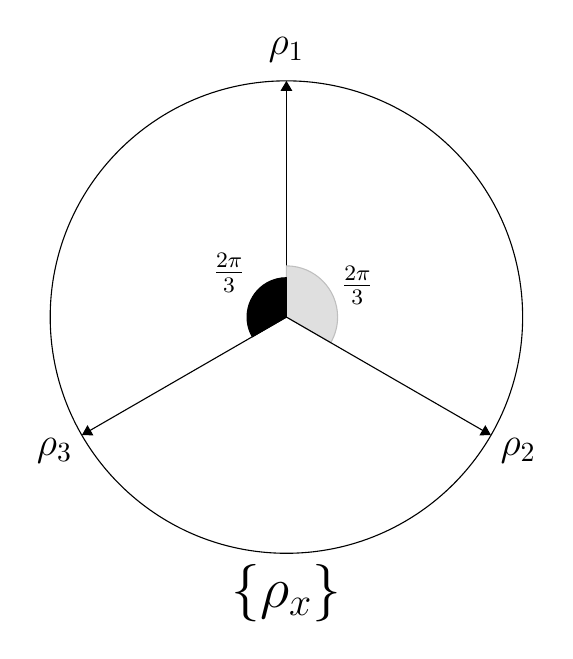
\begin{tikzpicture}[line cap=round, line join=round, >=Triangle]

\begin{scope}[ shift={(0,0)}]
\draw  (0,0) ellipse (3 and 3);


\draw[->]  (0,0) -- (0,3);
\draw (0,3.4) node {\Large $\rho_1$};
\draw [shift={(0,0)},lightgray, fill, fill opacity=0.5] (0,0) -- (90:0.65) arc (90:-30:0.65) -- cycle;
\node at (0.9,0.4) {\large $\frac{2\pi}{3}$};

\begin{scope}[rotate=120]
    \draw[->]  (0,0) -- (0,3);
	\draw (0,3.4) node {\Large $\rho_3$};
	
\draw [shift={(0,0)}, fill] (0,0) -- (90:0.5) arc (90:-30:0.5) -- cycle;
\node at (0.85,0.35) {\large $\frac{2\pi}{3}$};
\end{scope}

\begin{scope}[rotate=240]    
	\draw[->]  (0,0)  -- (0,3);
	\draw (0,3.4) node {\Large $\rho_2$};
\end{scope}
\node at (0,-3.5) {\huge $\{\rho_x\}$ };
\end{scope}


\end{tikzpicture}

\end{document}